
\section{Trilinears Coordinates}
\label{app:Atrilins}

The triangle is labeled in the usual (Euler's) manner: vertices $A$, $B$, $C$; angles $A$, $B$, $C$;
and sidelengths $a$, $b$, $c$: $a=|BC|,\; b =|AC|,\; c =|AB|$. If $X$ is a point in the plane of
the triangle $ABC$, then its position is completely determined by the ratios of directed distances (with signal)
from $X$ to the sidelines. Such ratios can therefore serve as coordinates for $X$.
Any ordered triple $[p, q,r]$ of numbers respectively proportional to the
directed distances (with signal) from $X$ to the sidelines $BC$, $CA$, $AB$ are called {\em  homogeneous trilinear coordinates}, or,  {\em  trilinears.}

\begin{figure}
    \centering
  % 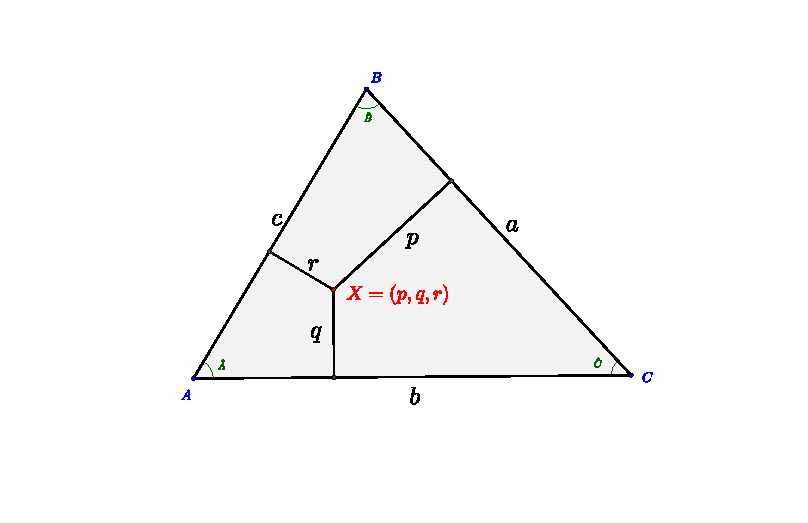
\includegraphics[scale=0.5]{trilinear.pdf}
 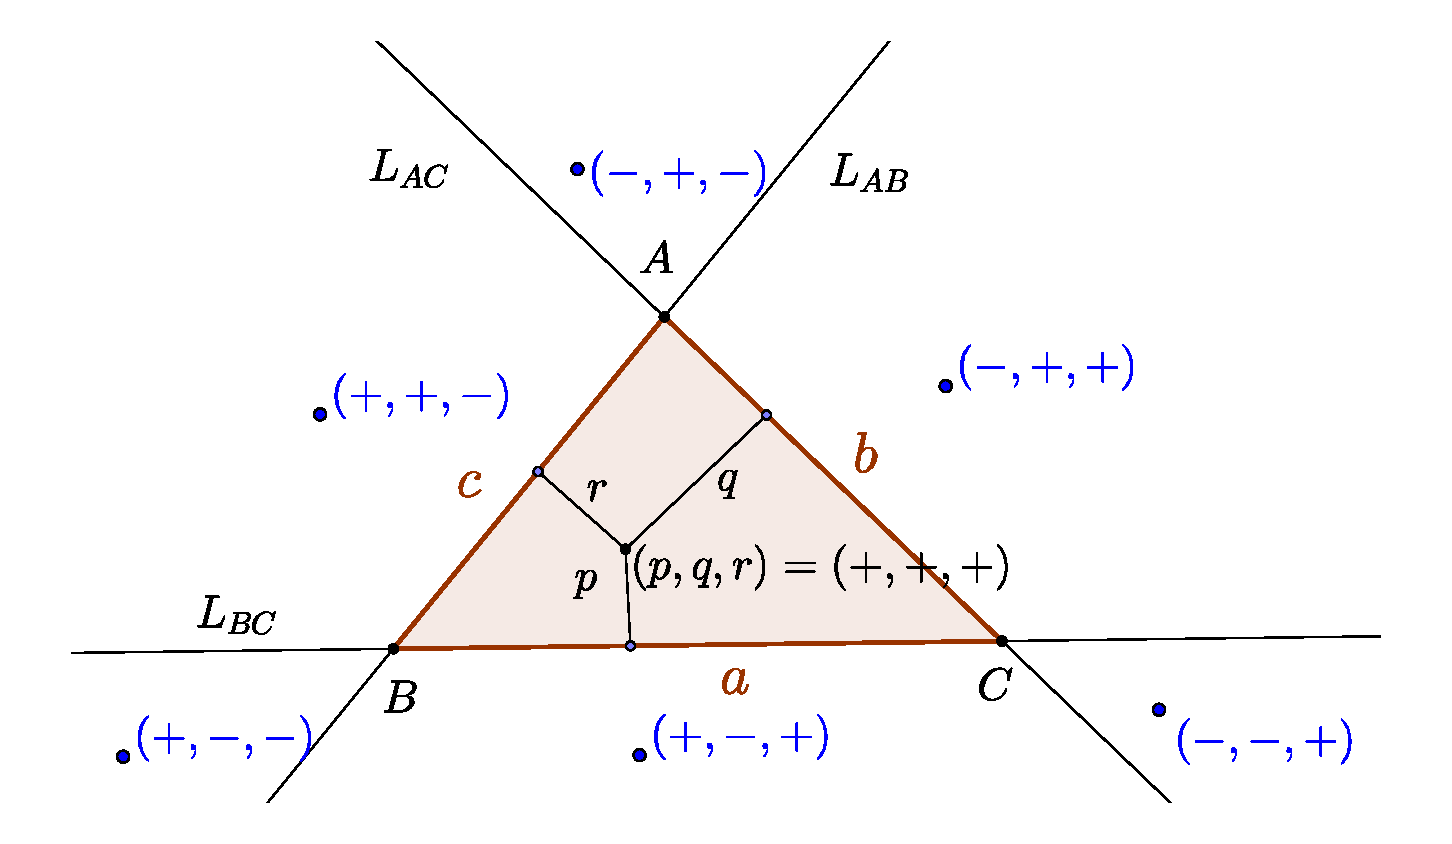
\includegraphics[scale=0.5]{zappA/pics/pics-appA-020-trilinear_signal.pdf}
    \caption{Trilinear coordinates in the plane.}
    \label{fig:trilinear_signal}
\end{figure}

Consider a point given in  homogeneous trilinear coordinates $[p,q,r]$.   Then   $k p,k q$ and $k r$, with
%
\[
k=\frac{2\Delta}{a p+b q+c q}
\]
are the directed distances (with signal) to the sidelines of the triangle $ABC$. This normalization is necessary  to      determine the position of the point in relation to reference triangle $ABC$. Otherwise, is more convenient to consider the homogeneous trilinear coordinates.

The trilinear coordinates of the vertices of a reference triangle are
\[ [\frac{2\Delta}{a},0,0],\;\;B=[ 
0,\frac{
	\Delta}{b} ,0],\;\; C=[
0,0,\frac{2\Delta}{c},0].
\]

The incenter, given by $[1,1,1]$ has equal distance to the sidelines given by $(a+b+c)/2\Delta$ that is equal to the radius of the incircle.